\documentclass[tikz]{standalone}
\usepackage{tikz}
\usetikzlibrary{bayesnet}
\begin{document}
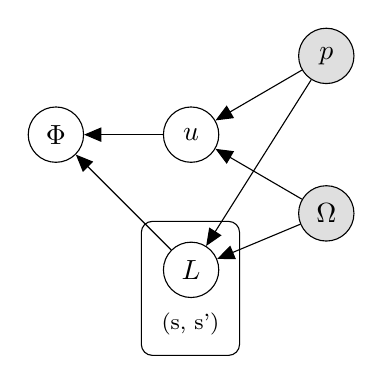
\begin{tikzpicture}

%Declare nodes.
\node[latent] (phi) {$\Phi$};
\node[latent, right=of phi] (u) {$u$};
\node[latent, below=of u] (L) {$L$};
\node[obs, right=of u, yshift=-1cm] (omega) {$\Omega$};
\node[obs, right=of u, yshift=1cm] (p) {$p$};

%Setup plates.
\plate[inner sep=0.25cm] {plate3} {(L)} {(s, s')};

%Setup edges.
\edge {omega, p} {u, L}
\edge {L} {phi}
\edge {u} {phi}

\end{tikzpicture}
\end{document}